\documentclass[final,20pt]{beamer}
% ====================
% Packages
% ====================

\usepackage[T1]{fontenc}
\usepackage{lmodern}
% change the orientation to landscape if needed
\usepackage[orientation=portrait,size=a0paper,scale=1.1]{beamerposter}
\usetheme{gemini}
\usecolortheme{uhb}
\usepackage{graphicx}
\usepackage{cleveref}
\usepackage[protrusion=true,expansion]{microtype}
\usepackage{booktabs}
\usepackage{tikz}
\usetikzlibrary{shapes.symbols}
\usetikzlibrary{shapes.arrows}
\usepackage{pgfplots}
\pgfplotsset{compat=1.18}
\usepackage{anyfontsize}
\usepackage[style=alphabetic,backend=biber]{biblatex}
\addbibresource{poster.bib}
\usepackage{wrapfig}
\usepackage{subcaption}
\usepackage{setspace}
% ====================
% Lengths
% ====================
% 1.5 Zeilenabstand
%\onehalfspacing%

% If you have N columns, choose \sepwidth and \colwidth such that
% (N+1)*\sepwidth + N*\colwidth = \paperwidth
\newlength{\blocksep}
\newlength{\sepwidth}
\newlength{\colwidth}
\setlength{\blocksep}{0.05\pageheight}
\setlength{\sepwidth}{0.025\paperwidth}
\setlength{\colwidth}{0.3\paperwidth}

\newcommand{\separatorcolumn}{\begin{column}{\sepwidth}\end{column}}

% ====================
% Title
% ====================

\title{Land Use Change and Climate Change Impact on \newline Urban Heat Islands Development}

\author{Linus Andrae\inst{1}}

\institute[shortinst]{\inst{1} Institute for Environmental Physics, University of Bremen}

% ====================
% Footer (optional)
% ====================

\footercontent{%

  \begin{columns}[t]
    \begin{column}{\colwidth+5cm}
      \begin{wrapfigure}{l}{6cm}     
        \centering
        \vspace{-2cm}
        \includegraphics[width=5cm]{figures/qrcode.eps}
      \end{wrapfigure}
      \href{https://github.com/paradx/PresTPoster/blob/main/poster.pdf}{The online version of this Poster: \\%
      https://github.com/paradx/PresTPoster/blob/main/poster.pdf} \vspace{1cm}
    \end{column}
    \begin{column}{\colwidth}
      \vfill
      PresT Winter Semester 2023/2024 \\ University Bremen \hfill
    \end{column}
    \separatorcolumn%
    \begin{column}{\colwidth}
      \vfill
      \href{mailto:landrae@uni-bremen.de}{contact: landrae@uni-bremen.de}\\
      \vspace{1em}
      Proudly made with \LaTeX%
    \end{column}
  \end{columns}
  }
% (can be left out to remove footer)

% ====================
% Logo (optional)
% ====================
% use this to include logos on the left and/or right side of the header:
\logoright{\includegraphics[height=5cm]{logos/logoIUP.png}}
\logoleft{\includegraphics[height=5cm]{logos/logo}}

% ===================
% Configuration of blocks
% ==================

\addtobeamertemplate{block begin}
  {}
  {\vspace{1ex plus 0.5ex minus 0.5ex} % Pads top of block
     % separates paragraphs in a block
   \setlength{\parskip}{24pt plus 1pt minus 1pt}%
   \begin{adjustwidth}{2cm}{2cm}
  }
\addtobeamertemplate{block end}
  {\end{adjustwidth}%
   \vspace{2ex plus 0.5ex minus 0.5ex}}% Pads bottom of block
  {\vspace{\blocksep}} % Seperates blocks from each other

\addtobeamertemplate{block alerted begin}
  {}
  {\vspace{1ex plus 0.5ex minus 0.5ex} % Pads top of block
     % separates paragraphs in a block
   \setlength{\parskip}{24pt plus 1pt minus 1pt}%
   \begin{adjustwidth}{2cm}{2cm}
  }
\addtobeamertemplate{block alerted end}
  {\end{adjustwidth}%
   \vspace{2ex plus 0.5ex minus 0.5ex}}% Pads bottom of block
  {\vspace{\blocksep}} % Seperates blocks from each other

\addtobeamertemplate{block example begin}
  {}
  {\vspace{1ex plus 0.5ex minus 0.5ex} % Pads top of block
     % separates paragraphs in a block
   \setlength{\parskip}{24pt plus 1pt minus 1pt}%
   \begin{adjustwidth}{2cm}{2cm}
  }
\addtobeamertemplate{block example end}
  {\end{adjustwidth}%
   \vspace{2ex plus 0.5ex minus 0.5ex}}% Pads bottom of block
  {\vspace{\blocksep}} % Seperates blocks from each other

% ====================
% Body
% ====================

\begin{document}

\begin{frame}[t]
\tikz[remember picture, overlay] \node[opacity=0.3, yshift=-1cm] at (current page.center){\includegraphics[width=\textwidth,height=0.99\textheight]{figures/overlay}};
\begin{columns}[t]
\separatorcolumn%

\begin{column}{\colwidth}

  \begin{alertblock}{Introduction}
    Urban Heat Islands are a phenomena where the temperature within a city is significantly higher within an urban area, compared to the temperature of the surrounding rural area. \\
    \begin{itemize}
      \item \textbf{Goal:} Detection of UHIs using Remote Sensing Satellite Data 
      \item \textbf{Why} Measure impact of different factors over time 
        \begin{itemize}
          \item land cover change
          \item temperature change 
        \end{itemize}
      \item \textbf{Output} Output factors and Indices of these factors on UHI severity and size
    \end{itemize}
  \end{alertblock}

  \begin{exampleblock}{Urban Heat Islands}
    \begin{itemize}
      \item \textbf{Urban Heat Islands} (UHIs) $\rightarrow$ surface and air temperature within a city is higher then the average temperature of the surrounding
      \item \textbf{Consequences} $\rightarrow$ Major health impact, increased pollution, reduced well-being 
      \item \textbf{Measuring} $\rightarrow$ Remote Sensing data and local weather station measurements 
    \end{itemize}
  \end{exampleblock}


  \begin{exampleblock}{Processing Chain}
   The Image Processing Pipeline can be separated in these steps:
    \begin{enumerate}
      \setlength\itemsep{1em}
      \item \textbf{Preprocessing} Cutting the image area to the Area of Interested
      \item \textbf{Feature Engineering} A Gabor filter bank of rotated Gabor kernels is used to enrich pixels with information about there place in larger structures of the image
      \item \textbf{Image Classification}  The pixels are classified using a random forest machine learning model that was trained using k-means based classification. 
      \item \textbf{Urban Area Detection} Classes indicating Urban Areas are identified and the buffer zones are build up around the areas to calculate a reference temperature.
      \item \textbf{Peri-Urban Area Clean-up} Larger settlement structures are masked away in the surrounding areas
      \item \textbf{Detection of Urban Heat Islands} use thermal infrared channels to detect UHIs within the Urban Area
      \item \textbf{Statistical Analysis of UHIs} Pixel within the UHI are evaluated using land surface type, NDVI and NDBI indices
      \item \textbf{Timeline Creation} Repetition of the pipeline for different images of the same area over multiple years: 
        \begin{itemize}
          \setlength\itemsep{0em}
          \item change in size of UHIs 
          \item statistical composition of UHIs 
        \end{itemize}
      \setlength\itemsep{1em}
      \item \textbf{Climate Change Impact} Estimation of the impact of rising average temperatures: 
        \begin{itemize}
          \setlength\itemsep{0em}
          \item subtracting impact of metrological factors on size and intensity of UHIs
          \item subtracting impact of surface change on size and intensity of UHIs
        \end{itemize}
      \setlength\itemsep{1em}
      \item \textbf{Result} Correlating of UHI with climate and land use change 
    \end{enumerate}
  \end{exampleblock}

\end{column}

\separatorcolumn%

\begin{column}{\colwidth}
  \begin{block}{Feature Engineering}
  For adding information of surrounding larger scale structures to each pixels, for each image band the same bank of Gabor-filters was used. 
  \begin{itemize}
    \item \textbf{Gabor filter}$\rightarrow$ convolution of a sinosoid and a gaussian.
    \item \textbf{parameter variation} $\sigma$ of gaussian, $\nu$, $\lambda$ and $\phi$ of sine
    \item \textbf{Output} Detection of patterns, structures and textures in different orientations and sizes
    \item \textbf{Additional information} one binary marker if pixel is part of larger structure
  \end{itemize}
  The filter used in \cref{fig:feats} was rotated \textbf{5} times. \\ 
  Increasing the data from \textbf{8} color bands to \textbf{144} color and feature bands.
     \begin{figure}
       \begin{subfigure}{0.47\linewidth}
      \centering
      \includegraphics[width=0.9\linewidth]{figures/gabor}
      \subcaption{Example filter bank of 16 rotated Gabor-kernels~\cite{mediumgabor}} 
    \end{subfigure}
    \begin{subfigure}{0.47\linewidth}
      \centering
      \includegraphics[width=0.85\linewidth]{figures/features}
      \subcaption{Features extracted from an image of the city of Bremen\label{fig:feats}}
    \end{subfigure}
    \end{figure}
  \end{block}

\begin{tikzpicture}
  \node[overlay, remember picture, style=single arrow, fill=UHBRed, shape border rotate=270, minimum width=3cm , minimum height=2.6cm, yshift=2.2cm ,xshift=0.5\colwidth]{};
\end{tikzpicture}

  \begin{block}{Surface Classification}
    Using K means the surface classes seen in \cref{fig:classes} where determined.
    \vspace{-.6em}
    \begin{figure}
      \begin{subfigure}{0.9\textwidth}
        \centering
        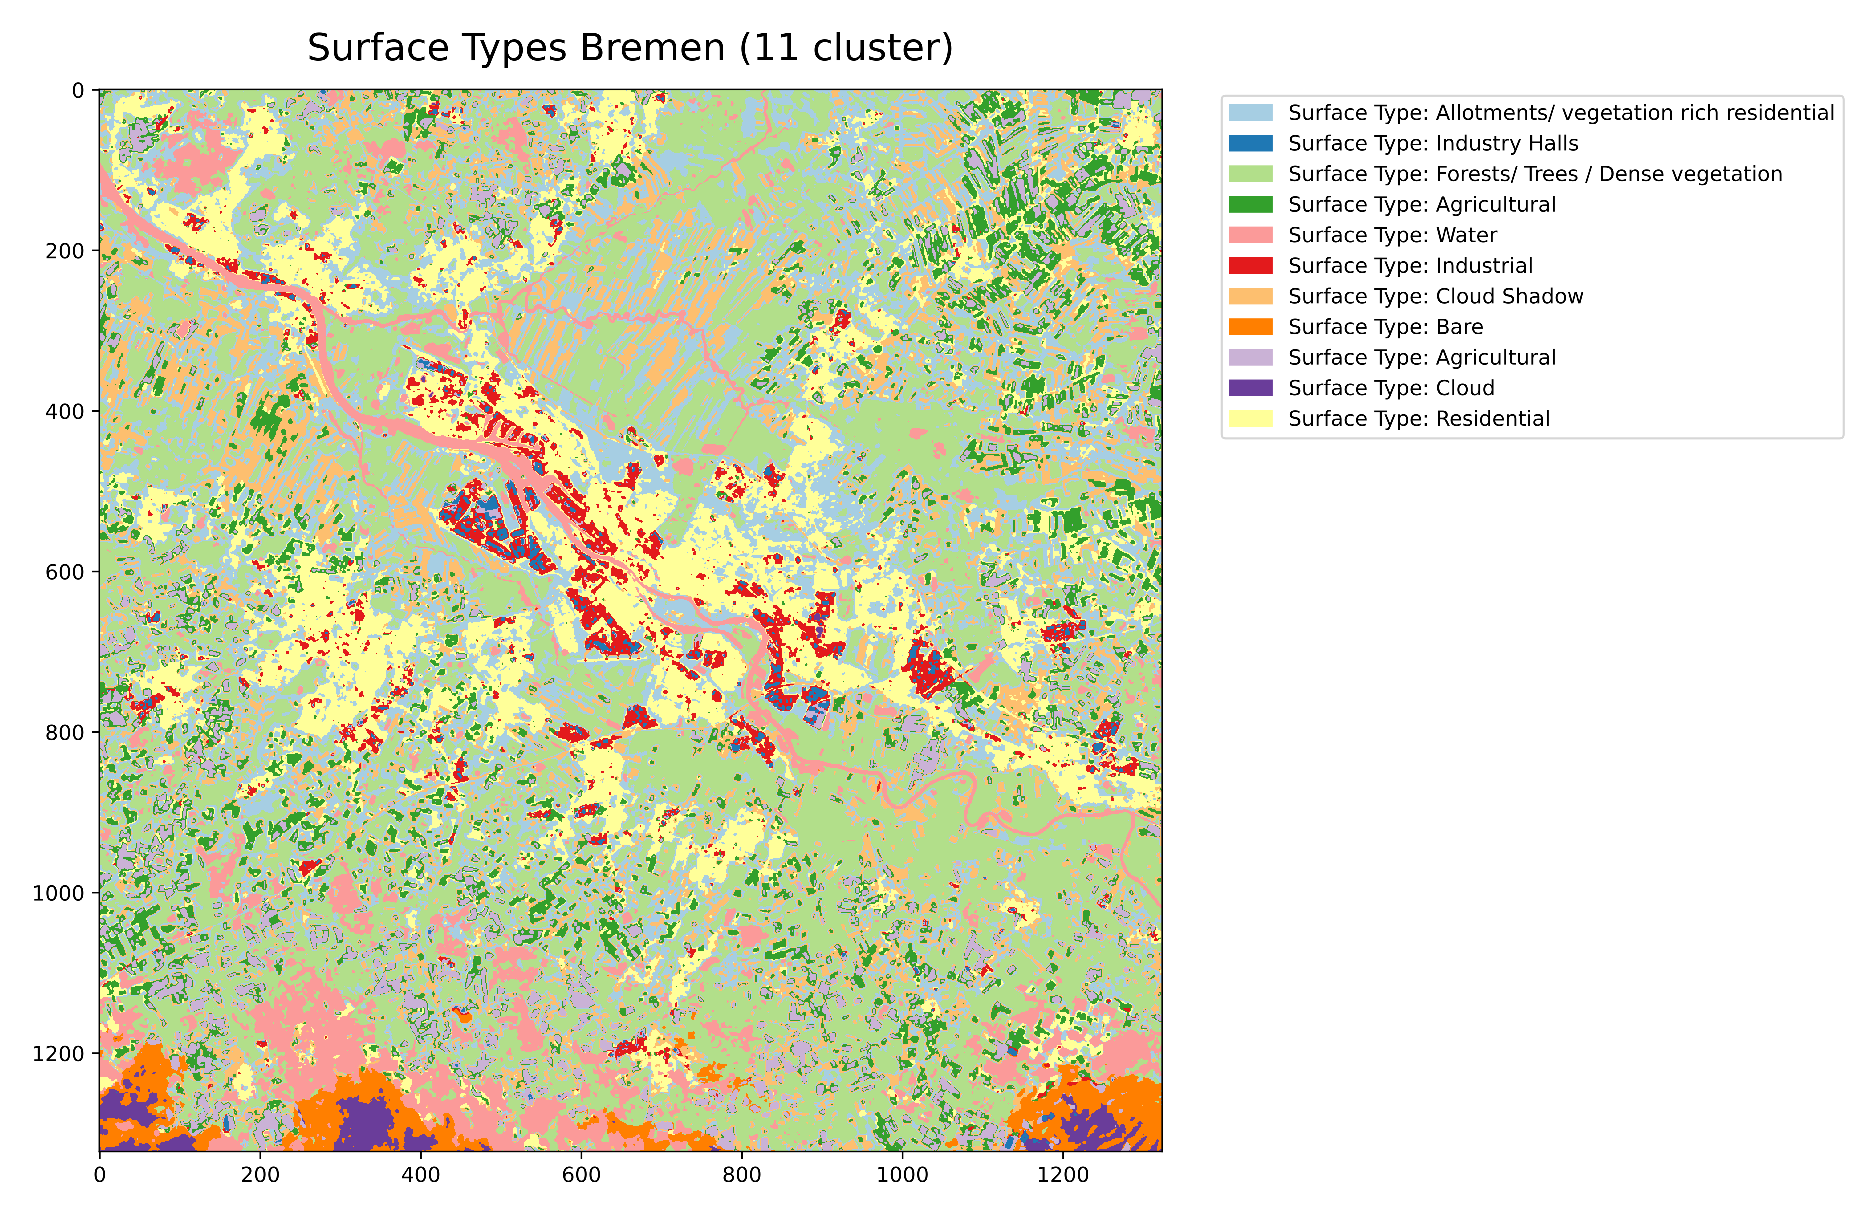
\includegraphics[width=\textwidth]{figures/classesBremen}
        \subcaption{Surface type classification of Bremen and the surrounding area\label{fig:classes}} 
      \end{subfigure}

      \vspace{-0.2em}
      \begin{subfigure}{0.9\textwidth}
        \centering
      \includegraphics[width=\textwidth]{figures/surroundingareas}
      \subcaption{Bremen urban area and the rural buffer zones\label{fig:urban}}
    \end{subfigure}
    \vspace{-2cm}
    \caption{Classification and urban area detection results}
  \end{figure}
  The Urban pixels where merged into a urban area with buffer and suburban zones (\cref{fig:urban}).\\
  \vspace{-1.5em}
  \begin{tikzpicture}
   \node[overlay, style=single arrow, fill=UHBRed, shape border rotate=270, minimum width=3cm, minimum height=2.6cm, yshift=-2.5cm, xshift=0.5\linewidth]{};
  \end{tikzpicture}
  \end{block}
\end{column}

\separatorcolumn%

\begin{column}{\colwidth}

\begin{tikzpicture}
   \node[overlay, style=single arrow, fill=UHBRed, shape border rotate=270, minimum width=3cm, minimum height=2.6cm, yshift=1.8cm ,xshift=0.5\colwidth]{};
\end{tikzpicture}
  
\vspace{1em}
  \begin{block}{UHI Detection}
  \begin{figure}
      \centering
      \includegraphics[width=0.9\textwidth]{figures/uhis}
      \caption{Urban Heat Islands detected in Bremen (more then 1.5 $\sigma$ above average temp)\label{fig:uhis}}
  \end{figure}
  \end{block}

\vspace{1em}
  \begin{tikzpicture}
    \node[overlay, style=single arrow, fill=UHBRed, shape border rotate=270, minimum width=3cm , minimum height=2.6cm, yshift=2.5cm ,xshift=0.5\colwidth]{};
  \end{tikzpicture}

  \begin{block}{Analysis and Results}
    \begin{figure}
        \centering
        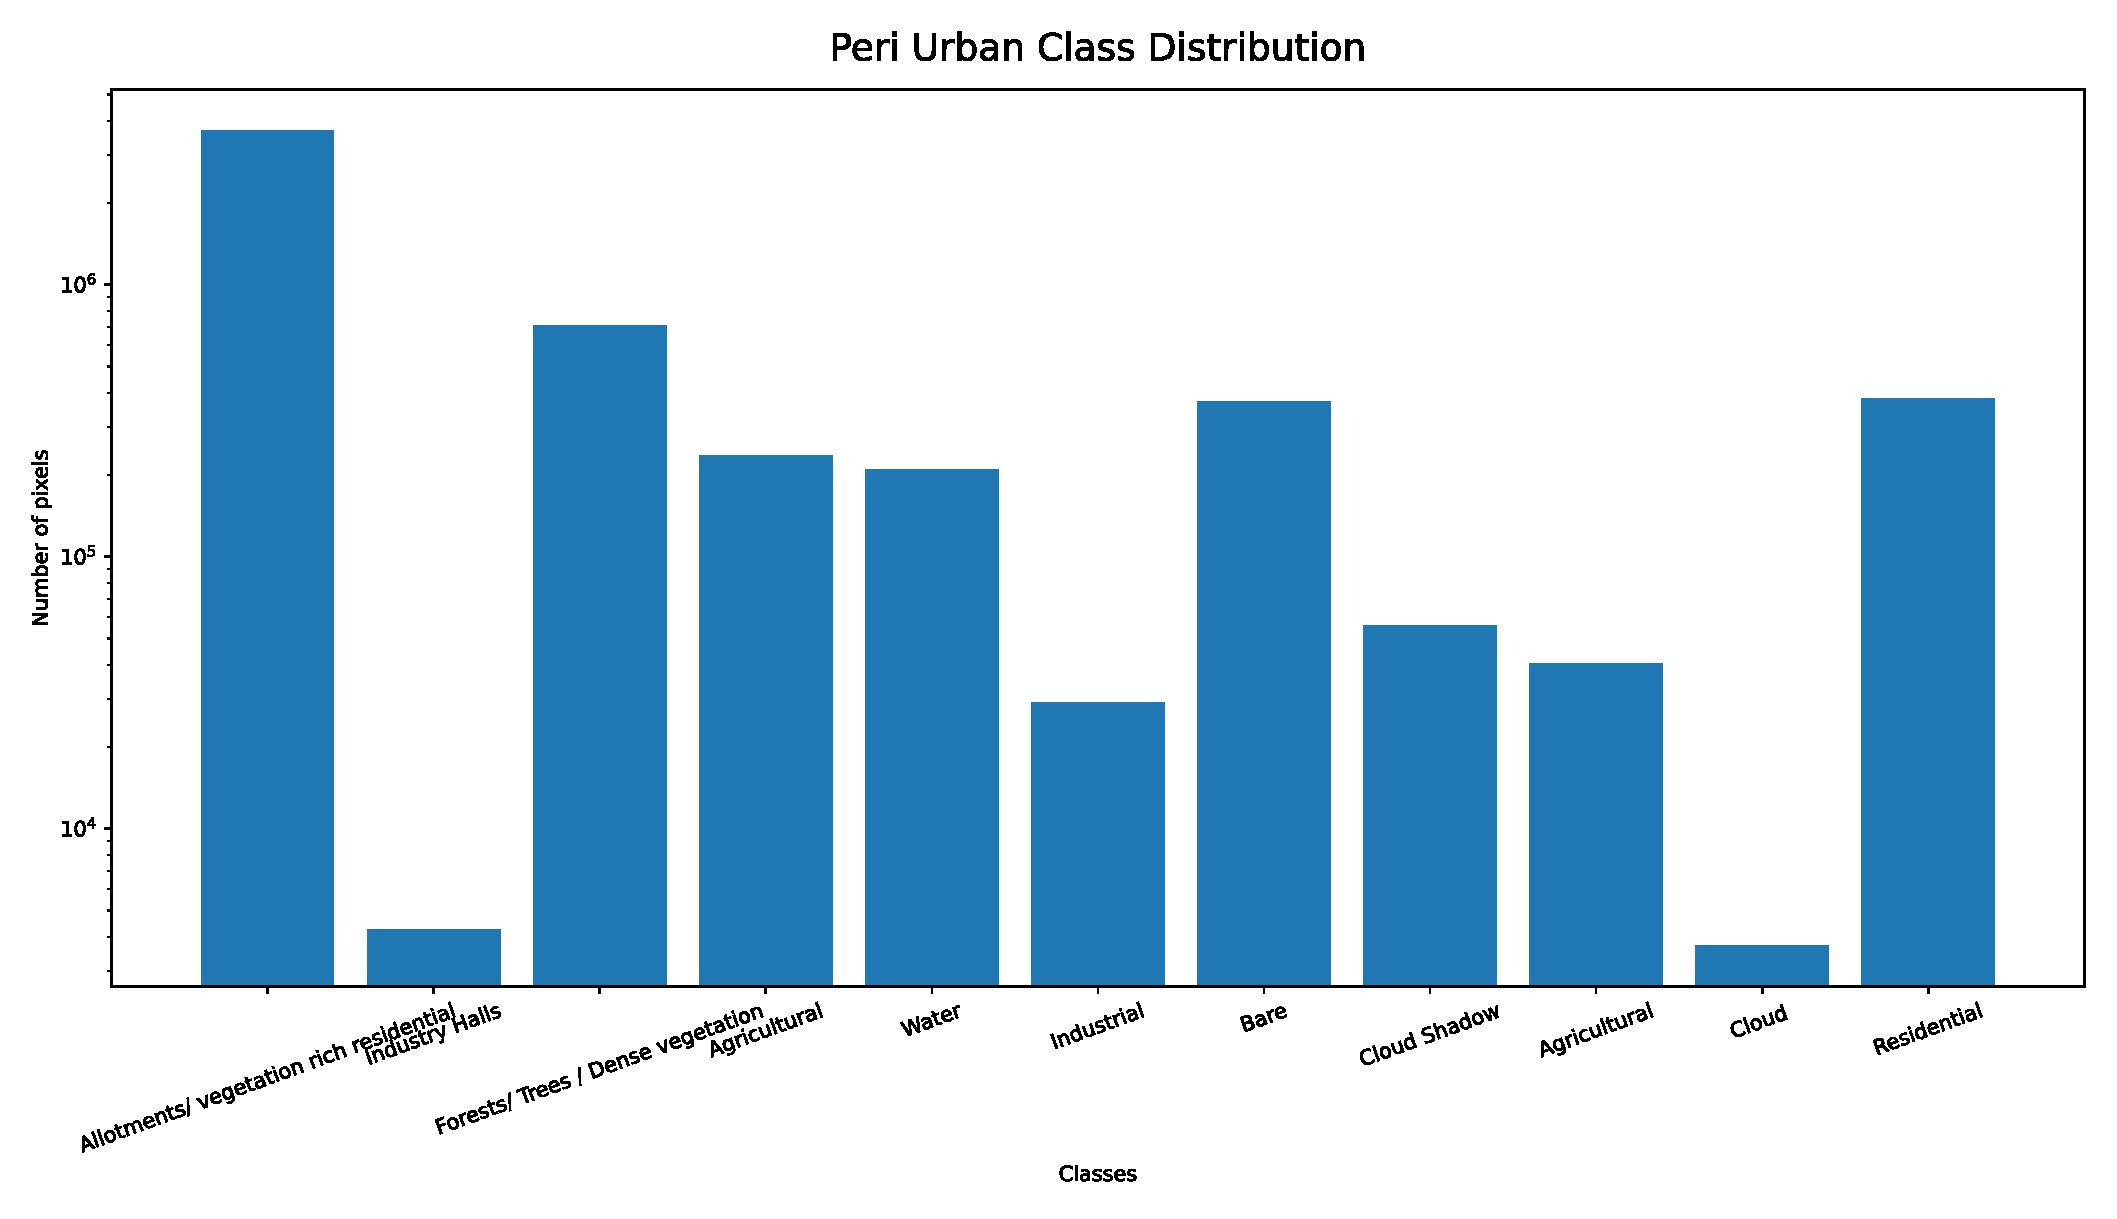
\includegraphics[width=\linewidth]{figures/PeriUrbanClassDistribution}
        \caption{Statistical analysis of the Bremen surface type distribution within the peri urban area}
    \end{figure}
    \begin{itemize}
      \setlength\itemsep{1em}
      \item City area classification works well with a combined approach
      \item Detecting Surface UHIs works well in different latitudes using Landsat 8 Satellite Images
      \item Severity depends highly on surface type and weather
      \item Climate Change and timeline analysis are currently a Work in Process (master thesis)
    \end{itemize}
  \end{block}

 % \begin{block}{Next Steps}
 %   \begin{itemize}
 %     \item Time Line
 %   \end{itemize}
 % \end{block}

  \begin{alertblock}{Summery}
    \begin{itemize}
      \setlength\itemsep{.2em}
      \item Remote Sensing Data can Help with detection and monitoring of UHIs
      \item UHIs pose a severe health risk
      \item UHIs pose a severe environmental risk
      \item Impact on humans will get worse with increased average temperatures
      \item Mitigation needs multidisciplinary approach
    \end{itemize}
  \end{alertblock}

  \begin{tikzpicture}
    \node[remember picture, overlay, starburst, fill=UHBYellow, draw=UHBRed, minimum width=6cm, line width=2pt, minimum height=4cm, rotate=20, yshift=16cm, xshift=7.5cm] {\bf TL;DR: };
  \end{tikzpicture}
  \vspace{-2em}
  \begin{block}{References}
    \nocite{*}
    \footnotesize{\printbibliography}
  \end{block}

\end{column}

\separatorcolumn%
\end{columns}
\end{frame}

\end{document}
% EOF
